\subsection{Discussion}

%%%%See if the discussion can be reorganized better%%%%%%%%%%%

As can be seen from the results above, according to the requirements and
resources available, each algorithm performs differently. Before
implementation, it is crucial to consider what resources are available and how
can a system be designed to obtain optimal results for those available
resources. Implementing the testbed framework on a cluster allowed us to
design, study and test the algorithms under realistic scenarios. We considered
different byzantine behaviors for each algorithm. To report on the number of
bits sent per process in the worst case, we considered byzantine processes that
try to flood the network. In this scenario, among the three algorithms we
considered, algorithm \textit{Pull-Push} performs the best generally. However,
in the case of a small network, with the number of processes less than $32$ and
a low fault percentage---(approximately less than $10\%$), algorithm
\textit{EIG} performs better since it considers the number of faults in its
protocol. 

If we were to consider a network with its size showing high variance over time,
algorithm \textit{Pull-Push} has the advantage that the number of bits sent per
node remains the same if the increase in size is within the next power of $2$.
For networks with strict bandwidth constraints, this allows high flexibility in
changing the size of the network. On the other hand, if we were to look at
networks which did not change in size but had varying fault ratios, algorithm
\textit{Quorum} inhibited a varying number of byzantine processes from changing
the communication complexity much. This, however, is restricted to networks
with high bandwidth in the first place. Our modified version of algorithm
\textit{EIG} showed this characteristic as well. The number of bits sent per
node increased very minimally on increasing the fault ratio and also performed
much better when compared to \textit{Quorum} or \textit{EIG} as can be seen in
Figure~\ref{fig:comp}.

Furthermore, we demonstrated a trade-off between the number of communication
bits and the number of rounds: algorithm \textit{Quorum} terminated in lower
number of rounds than \textit{Pull-Push} for all network sizes and fault
ratios. This can be attributed to its highly parallel protocol. Algorithm
\textit{EIG} displayed growth proportional to the size of the network, and
performed well only for very low fault ratios of $<10\%$. This trend are
reflected in the latency results as well when we consider the elapsed real
time. However, the total CPU time utilization increased rapidly for
\textit{Quorum} due to the exponential increase in the number of sub-protocols
executed in parallel as the network size increased.
\begin{figure}[ht]
 \centering
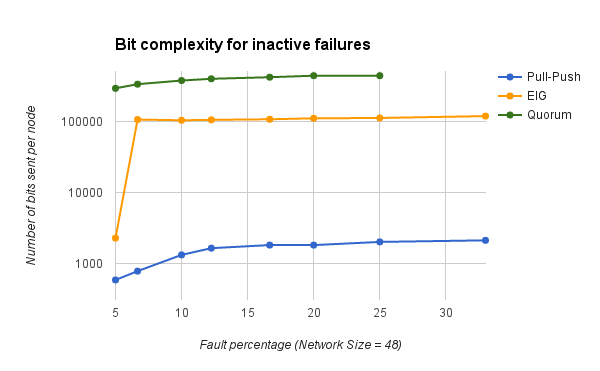
\includegraphics[scale=0.4]{crash}
\caption{Comparison for crash failures}
 \label{fig:crash}
\end{figure}

In the case of a denial of service attack, an increasing ratio of faulty processes reduced the communication overhead instead of increasing it. Similar results were also observed for crash failures. To evaluate the effect of crashes, we tested the system such that crash failures occurred on a uniform distribution over time. As can be seen in Fig. \ref{fig:crash}, an increasing fault ratio keeps the number of bits sent almost the same. If the faulty processes sent out only arbitrary messages, the algorithms executed correctly without hampering the communication cost much even if the ratio of byzantine processes was increased.

To further optimize the performance, one can improve certain tasks such as sending a larger message instead of many smaller messages or executing parallel tasks on multi-core machines. Another optimization that would have improved the running time of the system would be to use UDP connections instead of TCP since they take up less resources and provide lower overhead. Even though UDP connections do not guarantee message delivery, for a small system it could still be considered highly reliable. The rationale behind using TCP connections for our testbed framework was to model and understand implementation issues for more realistic distributed systems, which could have peers separated by geographical distance, requiring greater reliability. 

An analysis of the three algorithms and their performance for a wide range of number of processes and faults shows that communication of each process with fewer number of processes yields good results instead of all-to-all communication. This inhibits byzantine processes from influencing values of too many good processes. It is also important that requests from byzantine processes be throttled at an early stage. The good performance of the deterministic algorithm for small fault ratios shows that it is important to consider this factor when designing an algorithm.  Communication between multiple sets of quorums allows parallel tasks to be executed and gives good latency results. The combined use of these techniques would help design improved algorithms to solve the problem of distributed consensus. 



\section{Conclusion}
\label{sec:conc}
In real-world systems, achieving distributed consensus can be critically important. Consensus algorithms are used frequently in systems that rely on protocols such as those used in state machine replication and distributed databases. Thus, understanding the performance of algorithms for various scenarios occurring in real-time is essential to the overall performance of such systems. We show that there is a need to consider implementation issues that come along with any of these algorithms and not only their theoretical results. 

In this paper, we focused on implementation and analysis of three recently proposed algorithms with best results for their respective agendas. An Exponential Information Gathering protocol for consensus \cite{KM13} (algorithm \textit{EIG}) showed that deterministic algorithms have come a long way since the early results. We further improved upon the results obtained for this algorithm. In general, the randomized algorithm \textit{Pull-Push} \cite{BGH13}, performed better than the other two in terms of communication complexity. When latency was considered, as can be seen in Fig. \ref{fig:elapsed}, algorithm \textit{Quorum} \cite{BPV06} performed better. In real-time situations, as the number of processes in a network increase the probability of having faulty processes in the network naturally increases. Hence, even though algorithm \textit{EIG} shows better performance when the fault ratio is small, under high fault ratio its performance degrades. Quantifying the performance of the algorithms empirically provides a
practical understanding of how the different algorithms perform under
different conditions to achieve consensus in distributed systems.


\section{Acknowledgements}
We are grateful to Compute Canada for the use of computing resources and to NSERC for funding support.

\section{Vitae}

\begin{wrapfigure}{l}{0.3\textwidth}
    
\includegraphics[scale=0.4]{shreya.jpg}
\end{wrapfigure}

\textbf{Shreya Agrawal} completed her Master of Mathematics (Computer Science) from the University of Waterloo, Canada, in October, 2015. She graduated with a Bachelor of Technology degree in Information and Communication Technology from Dhirubhai Ambani Institute of Information and Communication Technology, India, in May, 2013. Her interests lie in theoretical computer science, more specifically in graph theory and formal logic, as well as distributed algorithms and cryptography. \\


\begin{wrapfigure}[4]{l}{0.3\textwidth}
    \vspace{-10pt}
    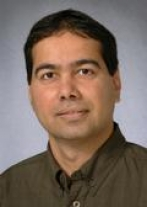
\includegraphics[scale=0.5]{kdaudjee.jpg}
\end{wrapfigure}

Khuzaima Daudjee is a faculty member in the Cheriton School of Computer
Science at the University of Waterloo. His research interests are in
distributed systems and data management.

